\section{Theorie}

\begin{align}
    \intertext{Unter der Millikan-Methode wird die Zerstäubung von Öltröpfchen in einem elektrischen Feld, welches durch einen Kondensator entsteht, verstanden, mit welcher die Elementarladung $e_{0}$ bestimmt wird.
    Bei der Zerstäubung laden sich dann die Tröpfchen elektrisch durch Reibung auf, um ganzzahlige Vielfache von $e_{0}$.
    Ohne ein angelegtes elektrisches Feld wirkt die Gravitationskraft auf das Tröpfchen $\vec{\text{F}}_{\text{g}} = \text{m}\vec{g} $.
    Die dabei entgegengerichtete Kraft ist die Stokesche-Reibungskraft, welche durch die Viskosität der Luft $\nu_{\text{L}}$ auftritt.
    Bei einem Gleichgewicht beider Kräfte wird das Tröpfchen nicht weiter beschleunigt}
    \frac{4\pi}{3}\text{r}^3 \left(\rho_{\text{Oel}} - \rho_{\text{L}}\right) \text{g} = 6\pi\, \eta_{\text{L}}\, \text{r}\, \text{v}_{0}\,, \label{1}
    \intertext{mit dem Tröpfchenradius r}
    r = \sqrt{\frac{9\,\eta_{\text{L}} \text{v}_0}{ 2\text{g} \left(\rho_{\text{Oel}} - \rho_{\text{L}}\right)} }\,. \label{2}
    \intertext{Beim Anlegen des elektrischen Feldes kommt eine wirkende Kraft hinzu, die elektrostatische Kraft $\vec{\text{F}}_{\text{el}} = \text{q}\vec{\text{E}}$.
    Diese Kraft wirkt immer in die Richtung des positiven Pols, wie in Abbildung \ref{Abbildung1} zu sehen.}
\end{align}

\begin{figure}[H]
    \centering
    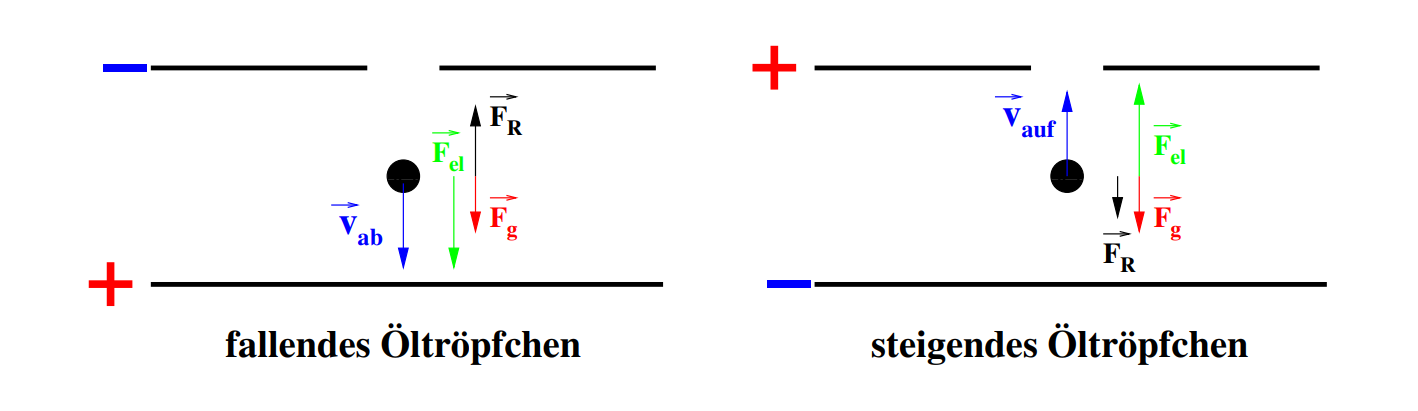
\includegraphics[width=130mm]{bilder/Abb1.png}
    \caption{Kräftegleichgewicht bei einem Tropfen in einem Plattenkondensator \cite{a1}. \label{Abbildung1} }
\end{figure}

\begin{align}
    \intertext{Wenn die elektrostatische Kraft in die selbe Richtung der Gravitationskraft zeigt, bewegt sich das Öltröpfchen mit einer schnelleren Geschwindigkeit $\vec{\text{v}}_{\text{ab}}$ als mit der Geschwindigkeit $\text{v}_{0}$ bei nicht angelegtem Feld.
    Dafür gilt}
    \frac{4\pi}{3}\text{r}^3 \left(\rho_{\text{Oel}} - \rho_{\text{L}}\right) \text{g} - 6\pi\, \eta_{\text{L}}\, \text{r} \text{v}_{\text{ab}} = -\text{q}\text{E}\,. \label{3} 
    \intertext{Wenn die Platten umgepolt werden, sodass die elektrostatische Kraft in die selbe Richtung der Reibungskraft zeigt und die Kraft ausreichend groß genug ist, bewegt sich das Tröpchen mit der Geschwindigkeit $\vec{\text{v}}_{\text{auf}}$ nach oben und es gilt}
    \frac{4\pi}{3}\text{r}^3 \left(\rho_{\text{Oel}} - \rho_{\text{L}}\right) \text{g} + 6\pi\, \eta_{\text{L}}\, \text{r} \text{v}_{\text{auf}} = +\text{q}\text{E}\,. \label{4}
\end{align}

\begin{align}
    \intertext{Durch die Gleichungen (\ref{3}) und (\ref{4}) lässt sich die Ladung q, die sich auf dem Tröpfchen befindet, mit dem dazugehörigen Tröpfchenradius r bestimmen}
    \text{q} = 3\,\pi\,\eta_{\text{L}}\,\sqrt{\frac{9\,\eta_{\text{L}}\, \left(\text{v}_{\text{ab}}-\text{v}_{\text{auf}}\right)}{4\,\text{g}\, \left(\rho_{\text{Oel}} - \rho_{\text{L}}\right)} } \cdot \frac{\text{v}_{\text{ab}}+\text{v}_{\text{auf}}}{\text{E}}\,, \label{5} 
\end{align}

\begin{equation} 
    \text{r} = \sqrt{\frac{9\,\eta_{\text{L}}\, \left(\text{v}_{\text{ab}}-\text{v}_{\text{auf}}\right)}{2\,\text{g}\, \left(\rho_{\text{Oel}} - \rho_{\text{L}}\right)} }\,. \label{6}
\end{equation}

\begin{align}
    \intertext{Mit Hilfe der Gleichung (\ref{5}) wird $\text{q}_{\text{unkorrigiert}}$, der Formel (\ref{6}) der Radius und mit der Formel }
    \text{q} = \text{q}_{0}\,\left( 1 + \frac{\text{B}}{\text{pr}} \right) \label{8}
    \intertext{wird $\text{q}_{\text{korrigiert}}$ berechnet.} \notag
\end{align}
